\documentclass[11pt]{article}

%Packages
\usepackage[a4paper, margin=1in]{geometry}

\usepackage{hyperref}
\usepackage{amsmath, amssymb}
\usepackage{siunitx}
\usepackage{romannum}

\usepackage{bookmark}
\usepackage{booktabs}
\usepackage{indentfirst}
\usepackage{multirow}
\usepackage{float}

\usepackage{titlesec}

\usepackage{graphicx}
\usepackage{subcaption}
\usepackage{tikz}
\usetikzlibrary{shapes.geometric, arrows, positioning}
\usepackage[american]{circuitikz}
\usepackage{listings}
\usepackage{xcolor}

\definecolor{codegreen}{rgb}{0,0.6,0}
\definecolor{codegray}{rgb}{0.5,0.5,0.5}
\definecolor{codepurple}{rgb}{0.58,0,0.82}
\definecolor{backcolour}{rgb}{0.95,0.95,0.92}

\lstdefinestyle{mystyle}{
    backgroundcolor=\color{backcolour},   
    commentstyle=\color{codegreen},
    keywordstyle=\color{magenta},
    numberstyle=\tiny\color{codegray},
    stringstyle=\color{codepurple},
    basicstyle=\ttfamily\footnotesize,
    breakatwhitespace=false,         
    breaklines=true,                 
    captionpos=b,                    
    keepspaces=true,                 
    numbers=left,                    
    numbersep=5pt,                  
    showspaces=false,                
    showstringspaces=false,
    showtabs=false,                  
    tabsize=2
}
\lstset{style=mystyle}

\newcommand*{\titleGP}{\begingroup
	\centering % Center all text
	\vspace*{\baselineskip} % White space at the top of the page

	\rule{\textwidth}{1.6pt}\vspace*{-\baselineskip}\vspace*{2pt} % Thick horizontal line
	\rule{\textwidth}{0.4pt}\\[\baselineskip] % Thin horizontal line
	{\LARGE Project Report}\\[0.2\baselineskip] % Title
	\rule{\textwidth}{0.4pt}\vspace*{-\baselineskip}\vspace{3.2pt} % Thin horizontal line
	\rule{\textwidth}{1.6pt}\\[2\baselineskip] % Thick horizontal line

	\vspace*{2in}
    
    	\Huge Precision Closed-Loop AC Power Controller using PID 
    	
	\vspace*{2in}
    

	\Large Name: Yojit Kumar\\
	\vspace*{0.2in}
	\Large Reg. No.: 20231289\\
	\vspace*{0.2in}
	\Large Course Code: PH3144\\
	\vspace*{0.2in}
	\Large Group: \#23\\

\endgroup}

\makeatletter
\let\latexps@plain\ps@plain
\newcommand{\frontmatter}{\let\ps@plain\ps@empty\pagestyle{empty}}
\newcommand{\mainmatter}{%
  \let\ps@plain\latexps@plain\pagestyle{plain}%
  \clearpage
  \pagenumbering{arabic}}
\makeatother

\begin{document}
\frontmatter
\titleGP
\clearpage

\mainmatter
\section{Introduction}
In any modern electric system, especially in labs, precise control over the power delivered to an electrical appliance/device is important for efficiency, stabilty and protection of devices. What we've tried to do is to precisely control the electrical power of any device. We are using a simple light bulb for the ease of demonstration. But in theory, we can implement this on any device connected to AC Mains.

Our device measures the current and voltage input for an electric load and allows us to fix a power in the working range of the appliance. We control this with a technique called \emph{phase-angle fired control}, where the firing  angle of a thyristor (Triac) is adjusted to control the portion of the AC Waveform delivered to the load.

For an electric bulb, this works as a dimmer for the system, allowing us to observe the difference. But a simple dimmer is an open-loop control, whilst we have implemented a closed-loop approach with help of \emph{PID}. You cannot ask the dimmer to set the bulb to run at $\SI{50}{\watt}$. You can only set it to 50\% effort, but you can't be sure. It is also susceptible to disturbances. If there is an increase in the voltage in the circuit, the dimmer doesn't know that, and the bulb will light brighter.

A closed-loop control is better because it uses the feedback to compare the result. We are constantly measuring the current and voltage to find the actual Power and compare it to the set-point to dynamically adjust the firing angle based on the feedback.

\section{Design}

\subsection{Block Diagram}
\begin{figure}[h!]
\centering
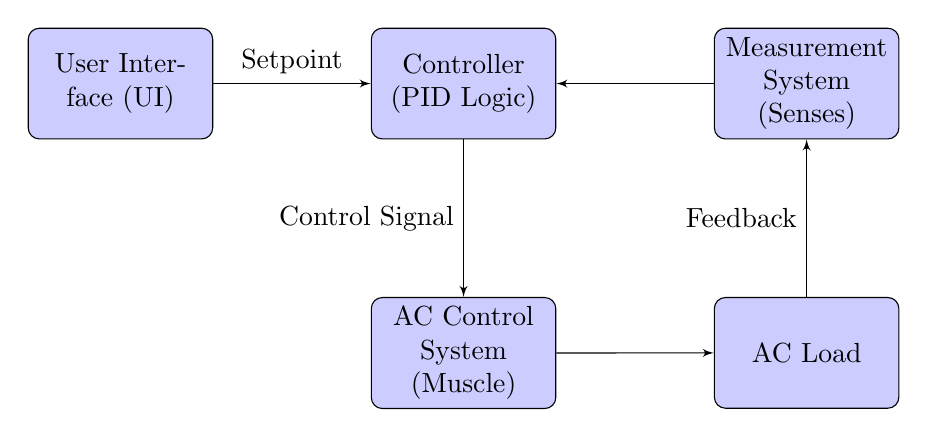
\begin{tikzpicture}[
    auto,
    block/.style={rectangle, draw, fill=blue!20, text width=6em, text centered, rounded corners, minimum height=4em},
    line/.style={draw, -latex'}
]

% Place the nodes
\node [block] (ui) {User Interface (UI)};
\node [block, right=2cm of ui] (arduino) {Controller (PID Logic)};
\node [block, below=2cm of arduino] (control) {AC Control System (Muscle)};
\node [block, right=2cm of arduino] (measure) {Measurement System (Senses)};
\node [block, below=2cm of measure] (load) {AC Load};

% Draw the lines (arrows)
\path [line] (ui) -- node [above] {Setpoint} (arduino);
\path [line] (arduino) -- node [left] {Control Signal} (control);
\path [line] (control) -- (load);
\path [line] (load) -- node [left] {Feedback} (measure);
\path [line] (measure) -- (arduino);

\end{tikzpicture}
\caption{Block Overview of the Closed-Loop Power Controller}
\label{fig:block_diagram}
\end{figure}

We divide our system into smaller task-specific parts to better understand our system. First is the User Interface (UI), it allows us to display the results and also fix a set-point for the system. The Controller (here Arduino) is the brain of the whole system, running the PID logic, and controlling all the other components of our project. The Measurement System consists of some simple sensors that allow us to take current and voltage measurements and send these to the Controller. The AC Control is the muscle of the system, it controls the parameters to maintain the set-point as dictated by the Controller.

\subsection{Hardware Design}

\begin{figure}[H]
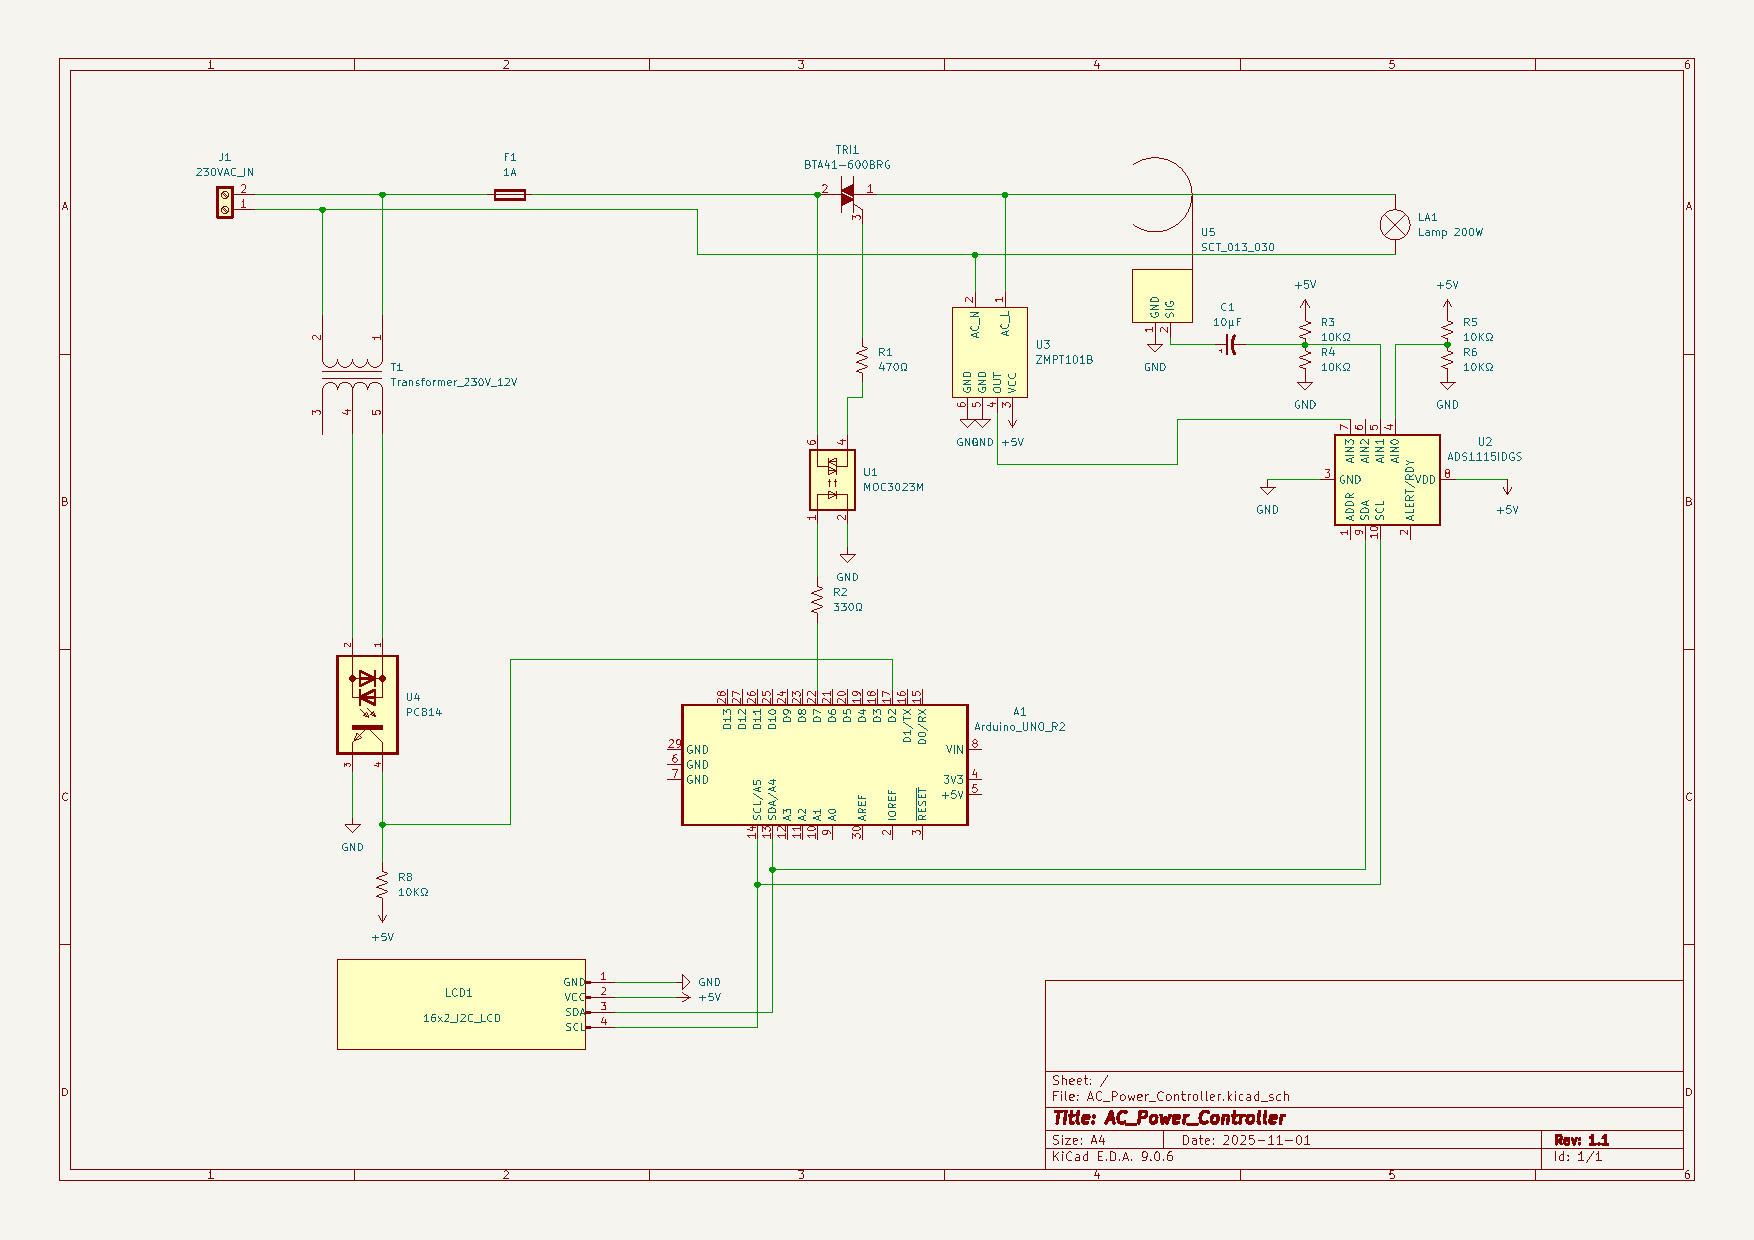
\includegraphics[width=\columnwidth]{AC_Power_Controller.pdf}
\caption{KiCad Schematics for the whole working the circuit}
\end{figure}

\subsubsection{Measurement Module}
This module is responsible for providing the critical feedback to the controller. The major components of the measurement module are:
\begin{enumerate}
	\item \underline{ZMPT101B Voltage Sensor Module}

		This active module safely steps down the $230\si{\volt}$ AC mains voltage to a low-voltage, isolated AC sine wave. Its onboard op-amp circuit biases this signal around a $2.5\si{volt}$ DC offset, making it safe for the low-voltage components to read.

	\item \underline{SCT-013-030 Current Sensor}

		A non-invasive current transformer that clamps around the live wire. It outputs a small AC voltage that is directly proportional to the AC current flowing to the load. This signal is also biased at $2.5\si{\volt}$ using an external voltage divider.

	\item \underline{ADS1115 16-bit  ADC Module}

		This is a high-precision, 16-bit Analog-to-Digital Converter. It is connected to the Arduino via the I2C bus (A4/A5). The Arduino's built-in 10-bit ADC is too noisy and has insufficient resolution for a "precision" controller. The 16-bit ADS1115 provides high-accuracy, low-noise measurements.
\end{enumerate}

\subsubsection{AC Control Module (Muscle)}
This component is the  high-voltage part of the circuit that controls the power flow. The major components that make up the AC Control Module are:
\begin{enumerate}
	\item \underline{MOC3023M (Triac Driver Optocoupler)}

		This chip is the safe bridge between the Arduino and the Triac. It receives a low-voltage $5\si{\volt}$ "fire" command from the Arduino (on pin D7) and uses an internal light-activated switch to trigger the high-voltage Triac.
		
		This provides galvanic isolation. It is the most important safety component, creating a physical air gap between the $230\si{\volt}$ AC circuit and the 5V logic circuit, protecting the Arduino and the user from lethal voltage.
	
	\item \underline{BTA41600B (Triac)}

		This is the heavy-duty, high-power AC switch. When it receives the trigger signal from the MOC3023M, it "latches" ON and conducts current to the light bulb. It automatically turns itself OFF (resets) at the end of every AC half-cycle when the current drops to zero.

		This is the component that actually controls the power. By precisely timing when this switch is turned on within each $10\si{\milli\second}$ half-cycle, we can control the total energy delivered to the load.

	\item \underline{PC814 (AC-Input Optocoupler)}

		This chip functions as our Zero-Crossing Detector (ZCD). Its AC input side watches the sine wave from the step-down transformer. At the precise moment the wave crosses its center point, the optocoupler's internal LED turns off, and triggers the phototransistor on the output side. This interrupt signal pulls down the output PIN\_4 that is connected to $+\SI{5}{\volt}$ of the Arduino.

		This signal is connected to the Arduino's hardware interrupt pin (D2). It provides a perfect timing pulse 100 times per second, synchronizing the Arduino's code with the AC line.	
\end{enumerate}

\section{Methodology}
In order to control the high-voltage current passing through the load to precisely change the power. We are using \emph{Phase Angle Control} using the \textbf{Triac}. The method requires us to change the gate voltage to the triac to control the current through the heavy load.
\begin{figure}[hbt]
	\centering
	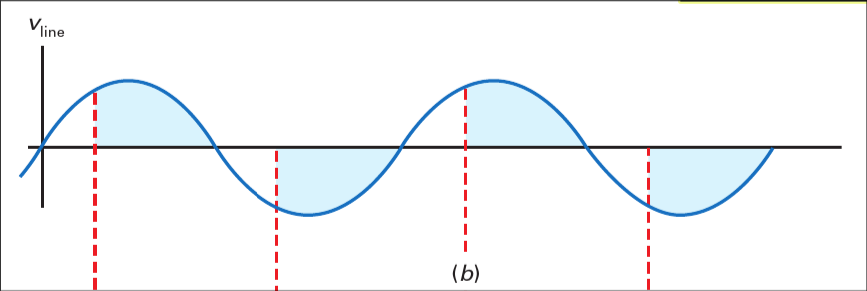
\includegraphics[width=0.75\columnwidth]{phase_angle_1.png}
	\caption{Line voltage for the triac \emph{Ref: Malvino \& Bates Pg. 549}}
	\label{fig:phase_angle_1}
\end{figure}

\begin{figure}[hbt]
	\centering
	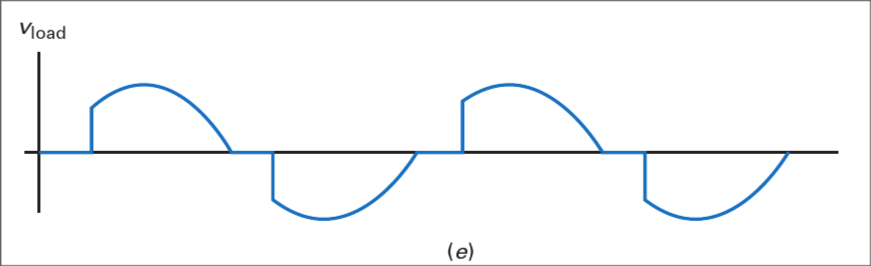
\includegraphics[width=0.75\columnwidth]{phase_angle_2.png}
	\caption{Voltage across a load connected to the triac \emph{Ref: Malvino \& Bates Pg. 549}}
	\label{fig:phase_angle_2}
\end{figure}

\autoref{fig:phase_angle_1} shows the line voltage. When the triac is triggered, the triac starts conducting. It basically means the triac is on, and it will remain on until the line voltage goes back to zero then it turns off again. \autoref{fig:phase_angle_2} shows us the voltage across the load during this process. This turning on and off happens for every half-pulse of AC passing through the triac. Thus, the triac is switches its state around 200 times a second.

\begin{figure}[hbt]
	\centering
	\begin{subfigure}[t]{0.5\textwidth}	
		\centering
		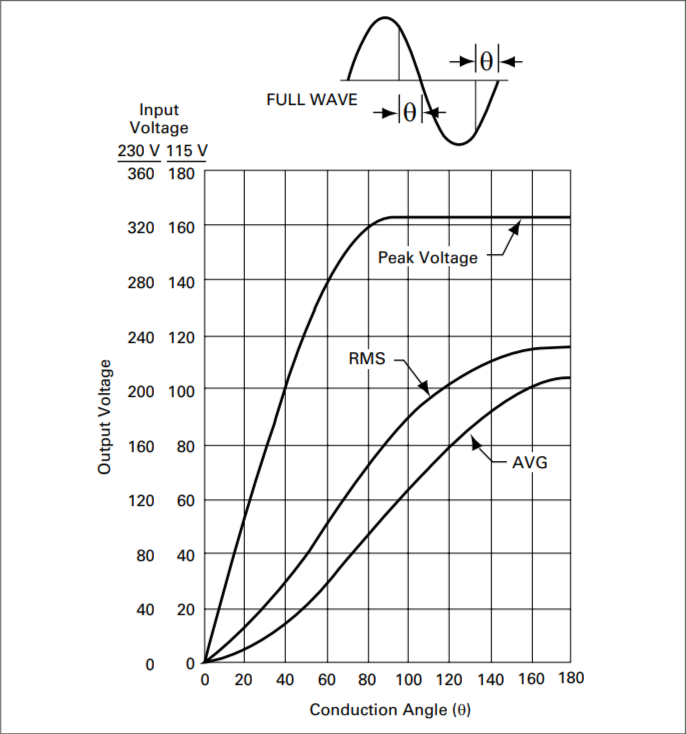
\includegraphics[width=0.99\linewidth]{output_voltage.png}
		\caption{Voltage of Full-Wave Phase Angle Control (Sinusodial)}
		\label{subfig:subfig_1}
	\end{subfigure}%
	\begin{subfigure}[t]{0.5\textwidth}
		\centering
		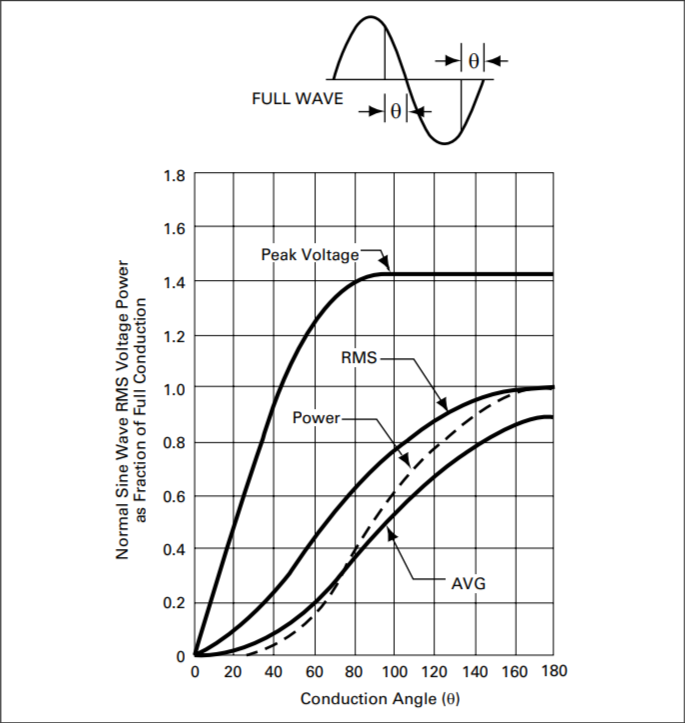
\includegraphics[width=1\linewidth]{output_power.png}
		\caption{Power of Full-Wave Phase Angle Control}
		\label{subfig:subfig_2}
	\end{subfigure}
	\caption{Voltage \& Power Curves for different $\theta$ \emph{Ref: Littlefuse AN1003 datasheet}} 
	\label{fig:power_curve}
\end{figure}

In \autoref{fig:power_curve}, $\theta$ is the conduction angle which is equivalent to $\pi - \theta_{\mathrm{firing}}$. $\theta_{\mathrm{firing}}$ is proportional to the firing delay. Thus, we can use the curves to study how the power or voltage may vary across the load as we change the firing delay.
But, as we are working with a closed-loop feedback system we don't need to refer to the curve, our algorithm is supposed to give us a correction just based on the error from the set point.

In order to find this error term, we need to find the real-time value of the power first. For which we are using a voltage sesing module (\emph{ZMPT101B}) and a current sensing module (\emph{SCT-013-030}), and both of these are connected to an external Analog-to-Digital Convertor(ADC) (\emph{ADS1115}) which is there to give us a better resolution than the onboard ADC of the Arduino Board.

Another important part of controlling the AC power and setting a firing delay is to actually know when the AC pulse starts. Because of how a triac functions it will auto turn-off at the end of each half cycle but we need to know the starting point. This starting point is detected using a zero-crossing detector that we have created using a step-down transformer and a AC input optocoupler (\emph{PC814}). We have also attached a basic I2C display to as a part of our user interface to display the power, voltage and current information in real-time.

\section{Implementation}

The project was designed with two separate perfboards:high-voltage perfboard as in \autoref{fig:high_voltage} and a low-voltage perfboard \autoref{fig:low_voltage}. This was created to keep in mind the safety of low volage components, and over safe handling of the project. We've also used optocouplers for the same reason; to create circuit isolation.

\begin{figure}[hbt]
	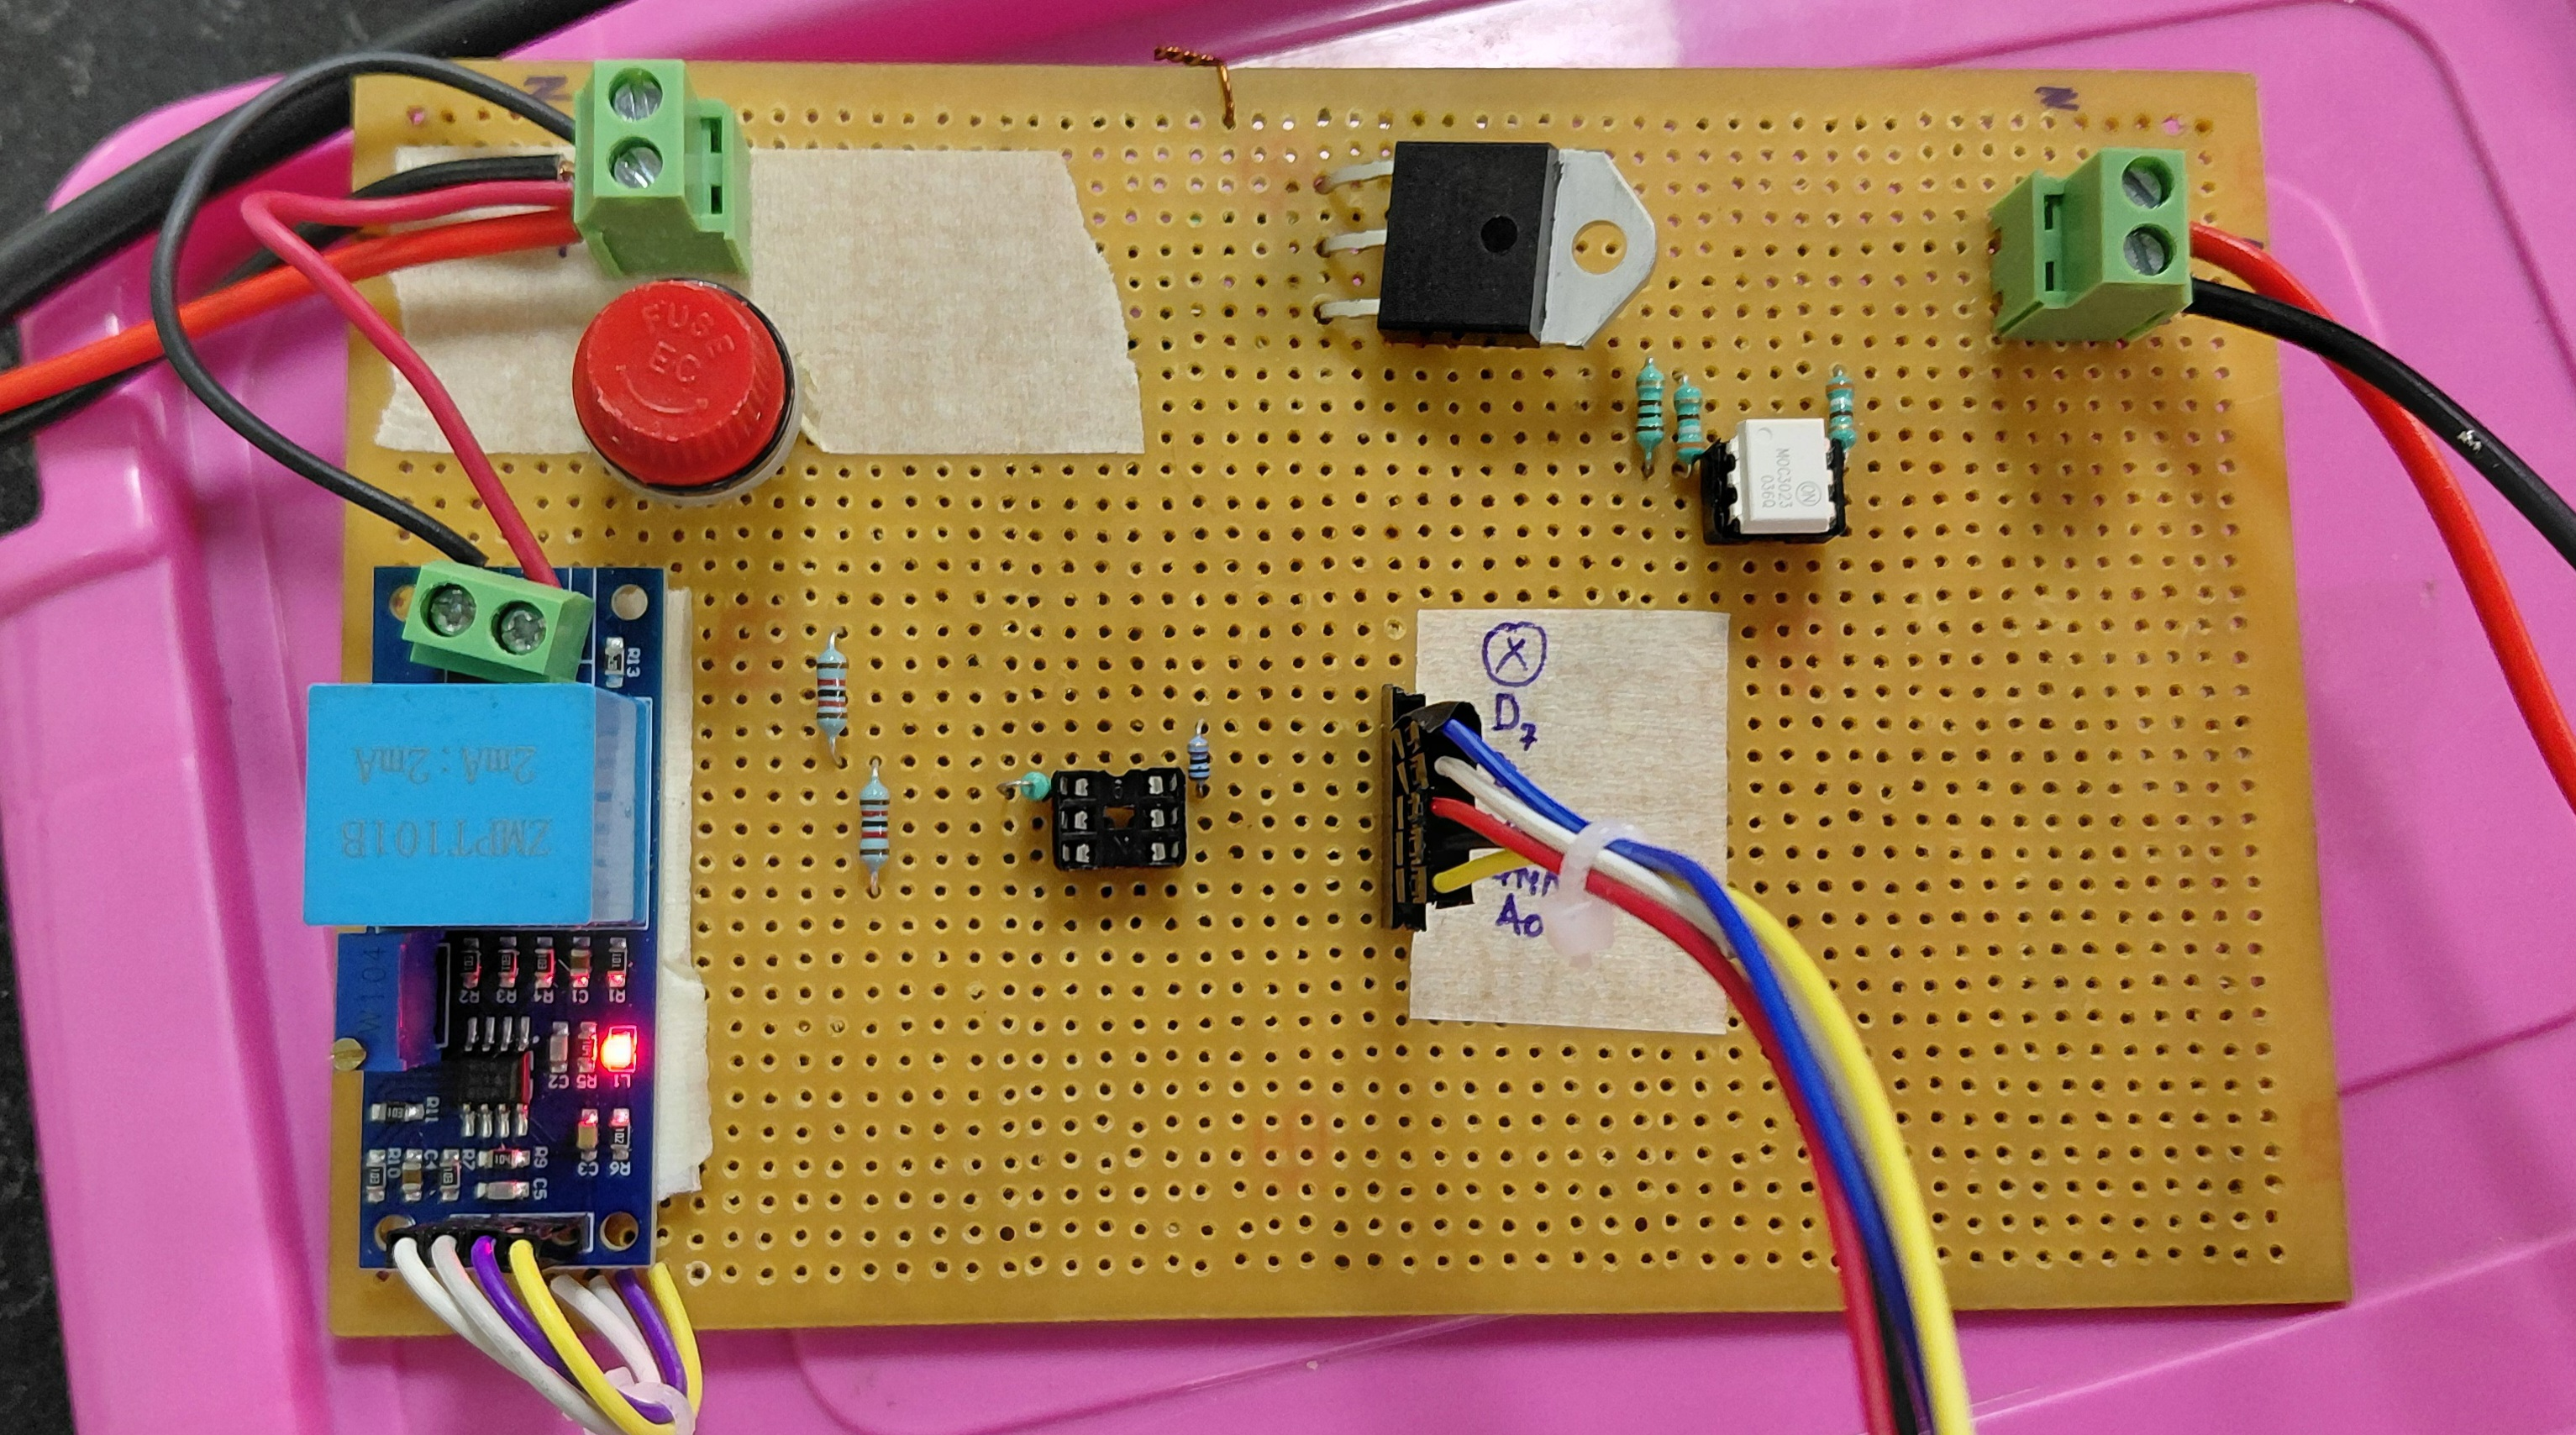
\includegraphics[width=\columnwidth]{20251113_150119 (1).jpg}
	\caption{\textbf{This is the high-voltage perfboard.} AC-In is from the left side which passes to the triac in the middle and load connected to the rightmost connetion point. Triac is connected to the \emph{MOC3023M} IC. The \emph{ZMPT101B} module at the left has a stepdown transformer visible to us as a blue cube. The empty IC base is supposed to hold the \emph{PC814} IC which is the AC input optocoupler, a part of the zero-crossing detector. All connections are soldered at the back and terminate at the jumper base in the middle, which we connect to the low voltage perfboard.}
	\label{fig:high_voltage}
\end{figure}

There is an extra component of the project on the breadboard as seen in \autoref{fig:zcd}. It is a zero-crossing detector made using \emph{PC814} IC and a bridge rectifier. The purpose of this circuit is to provide the required interrupt signal as seen in \autoref{fig:interrupt_signal}. This was created as a fix for a bug in our earlier designs. We will talk more on this in the debugging sections.

\begin{figure}[hbt]
	\begin{subfigure}[t]{0.45\textwidth}
	\flushleft
	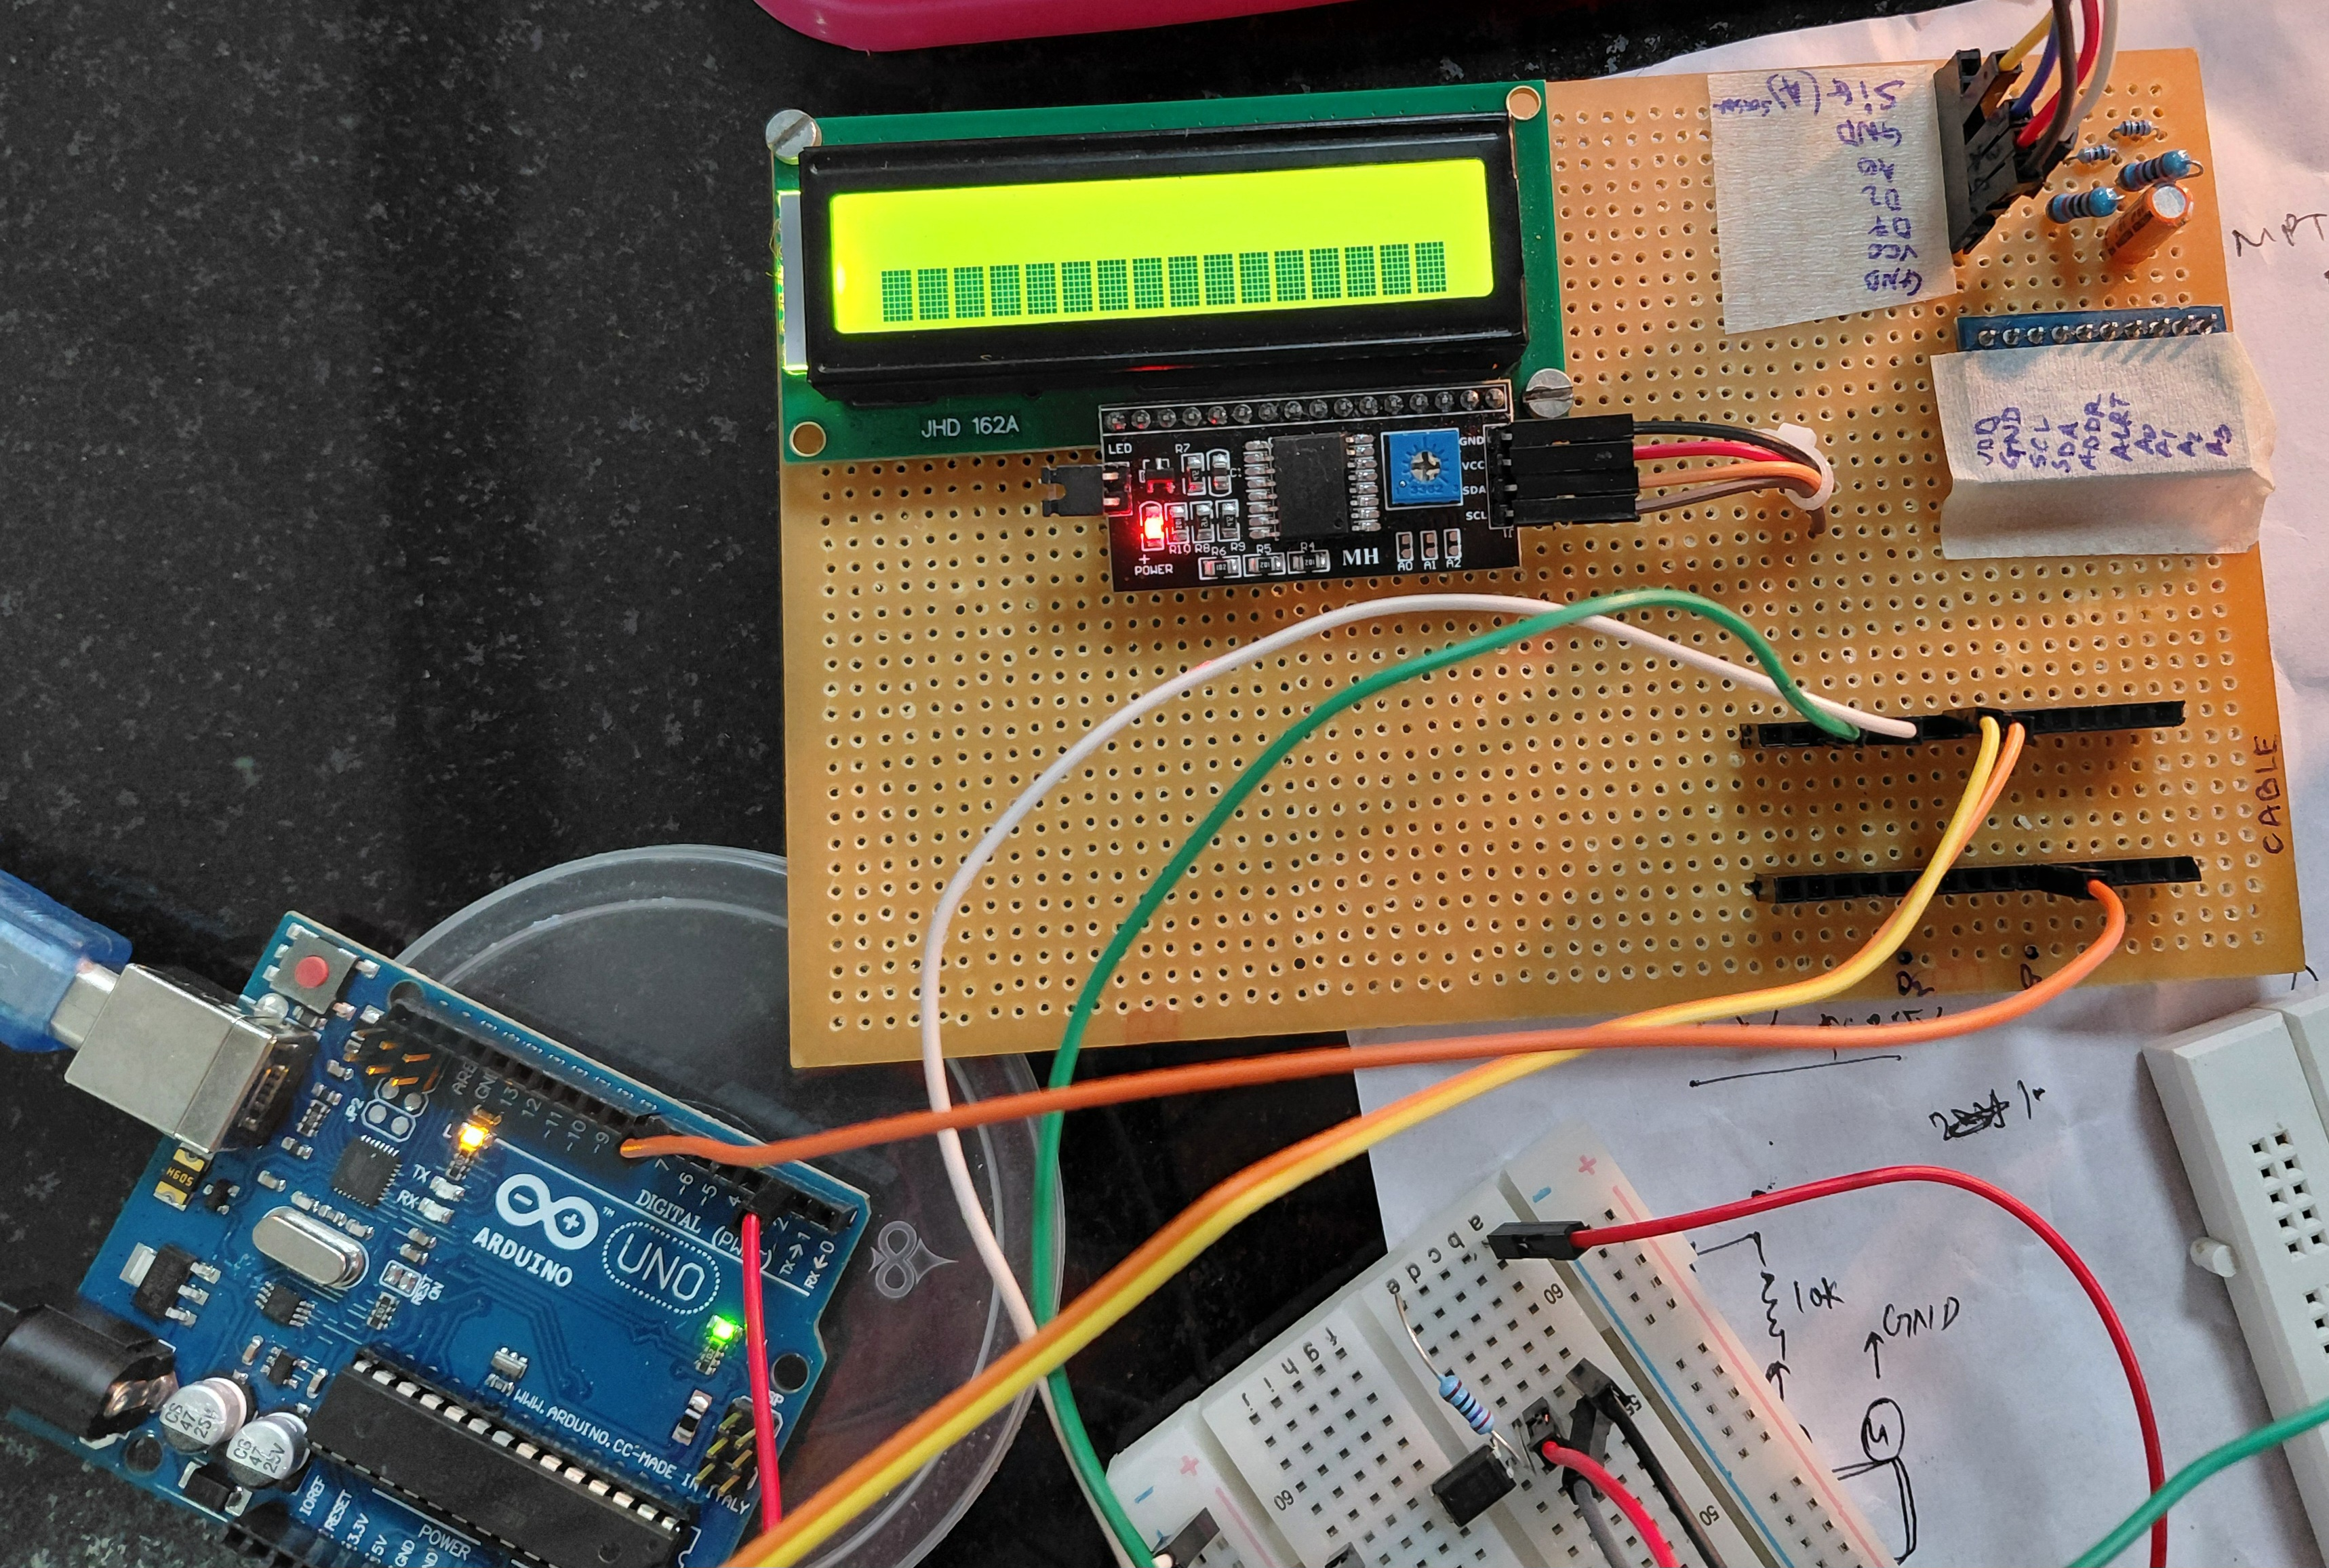
\includegraphics[width=0.85\textwidth]{20251113_150124 (1).jpg}
	\caption{\textbf{This is the low-voltage perfboard.} Jumper connections from the first perfboard and the current sensor module join at the top-right. There are voltage dividers and a clamper at the top for the ac-signal from the current-sensor module. The I2C display module is connected on top-left. And all connections terminate at the jumper base at the bottom, that connects to the \emph{Arduino UNO}}
	\label{fig:low_voltage}
	\end{subfigure}
	\hfill
	\begin{subfigure}[t]{0.45\textwidth}
	\flushright
	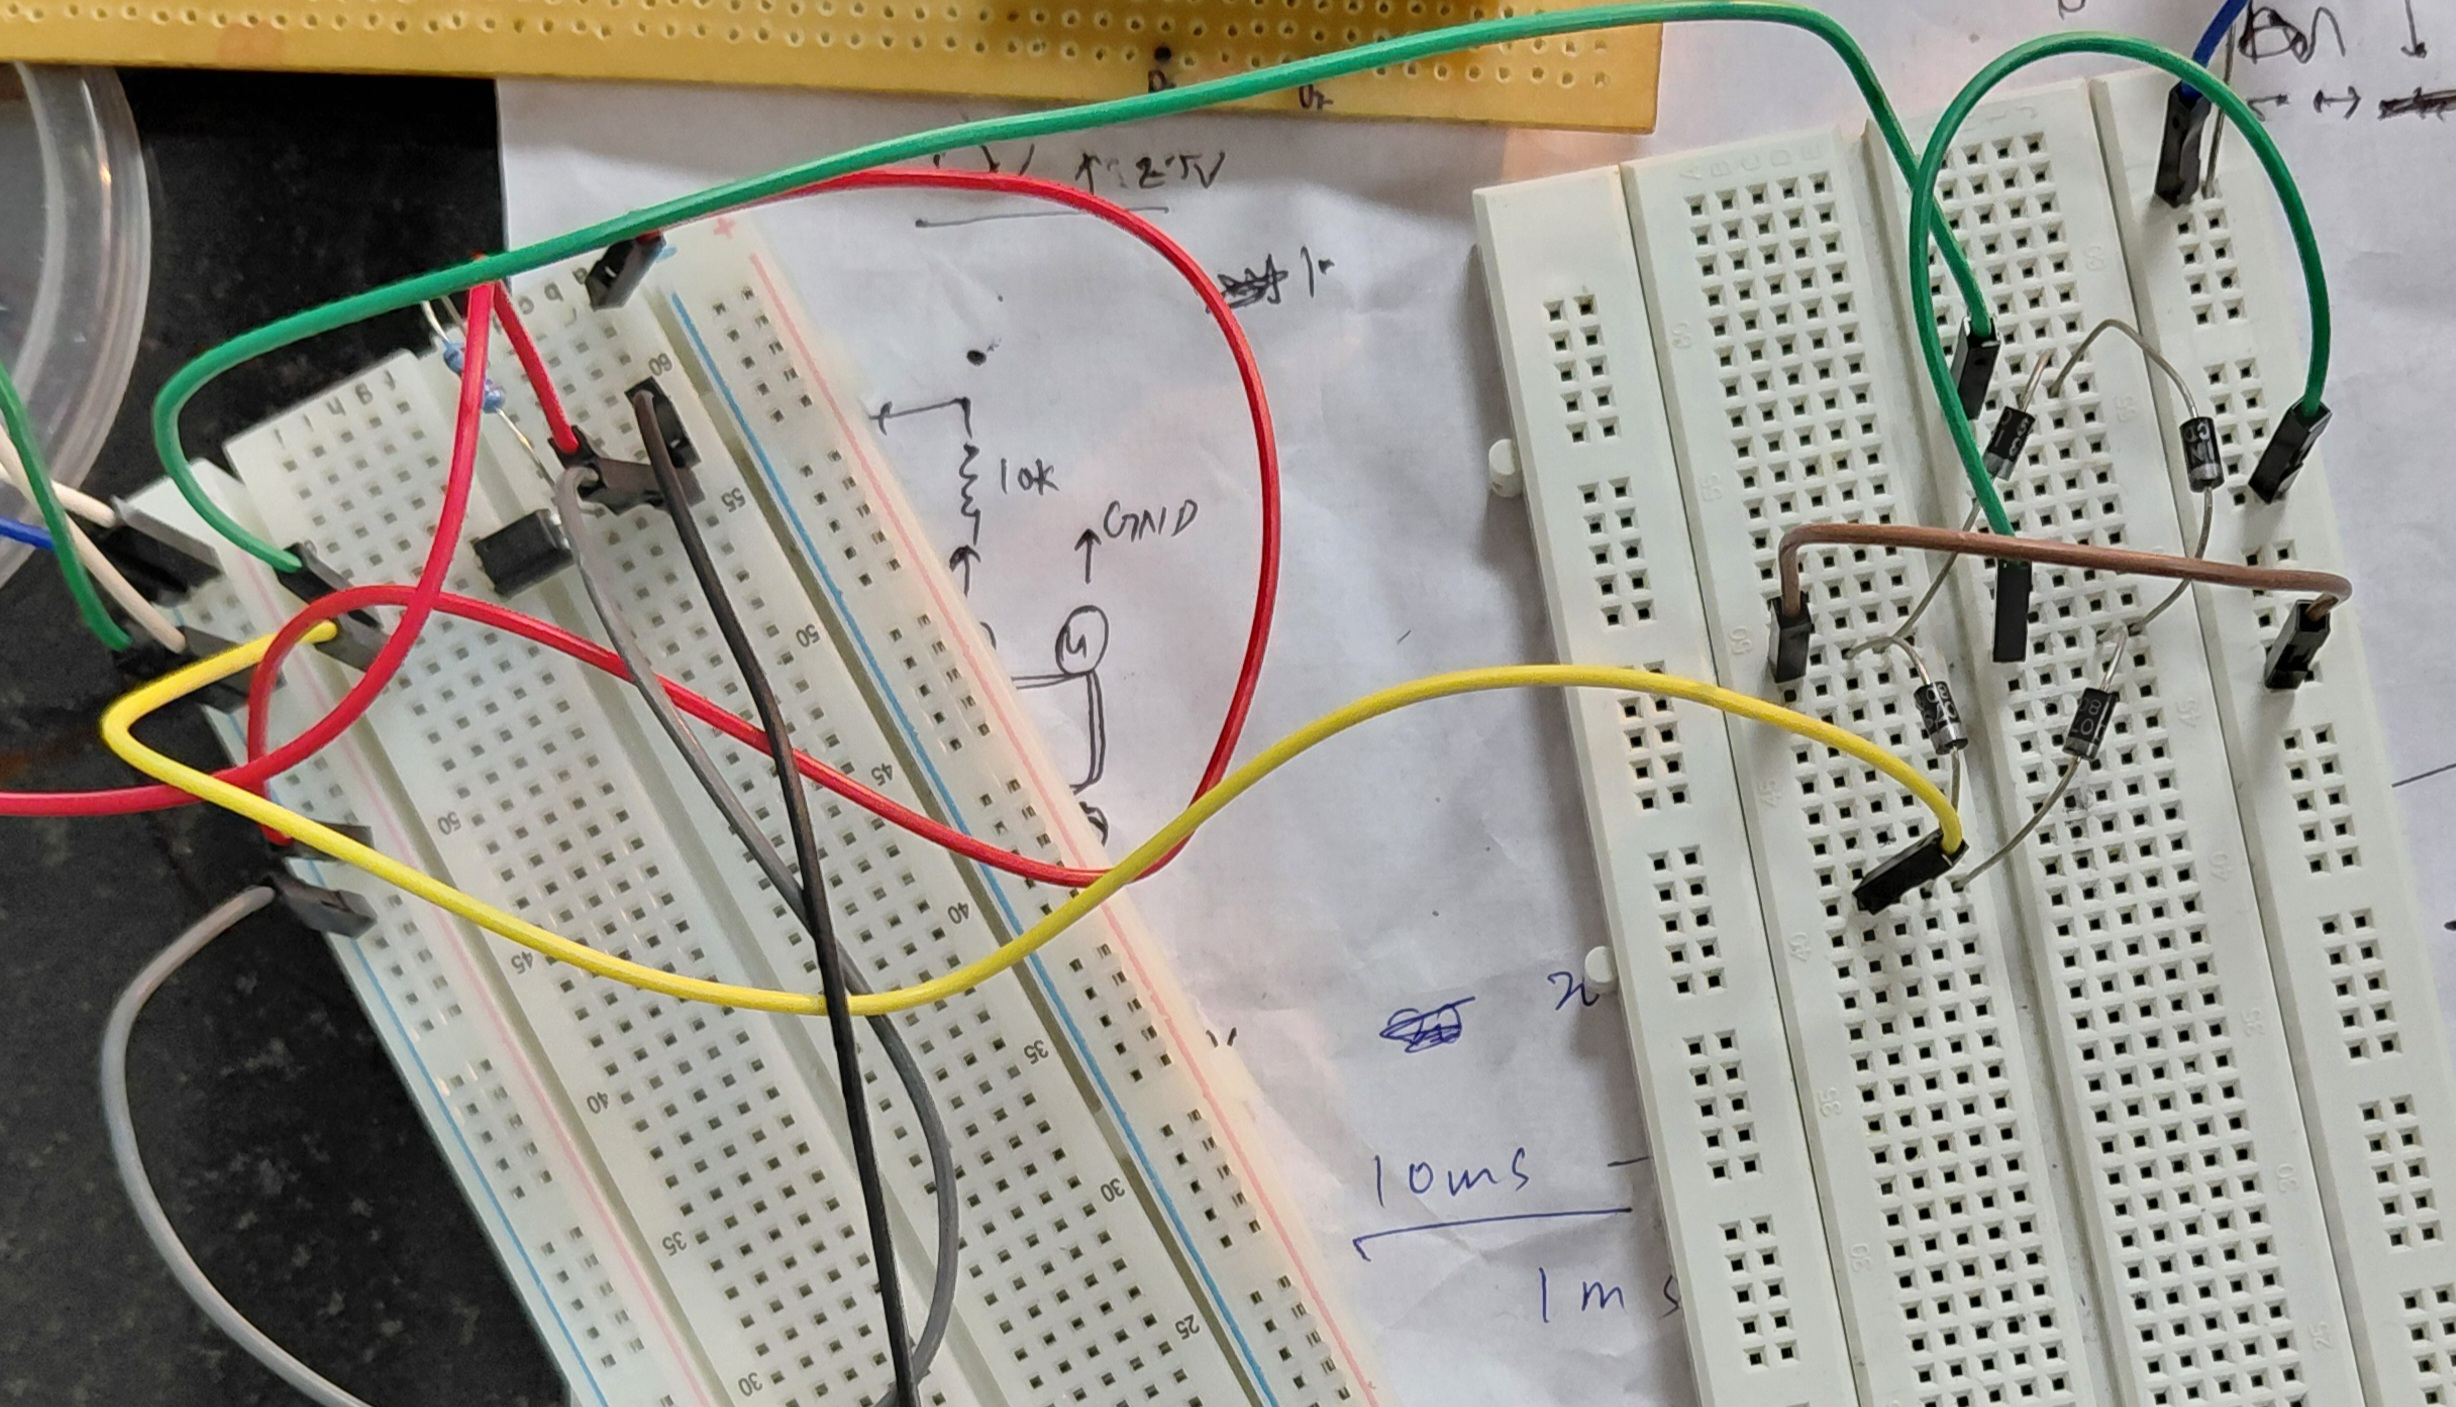
\includegraphics[width=\textwidth]{20251113_150127 (1).jpg}
	\caption{This is the zero-crossing detector fix we created. The right breadboard has a bridge-rectifier which is connected to a voltage output of a stepdown 12V transformer. The rectified signal is passing to the \emph{PC814} IC on the breadboard at the right. This simply triggers at the start of each pulse half-cycle and sends a signal to the \emph{Arduino UNO}}
	\label{fig:zcd}
	\end{subfigure}
	\caption{Low-voltage Circuit}
\end{figure}

\begin{figure}[hbt]
	\centering
	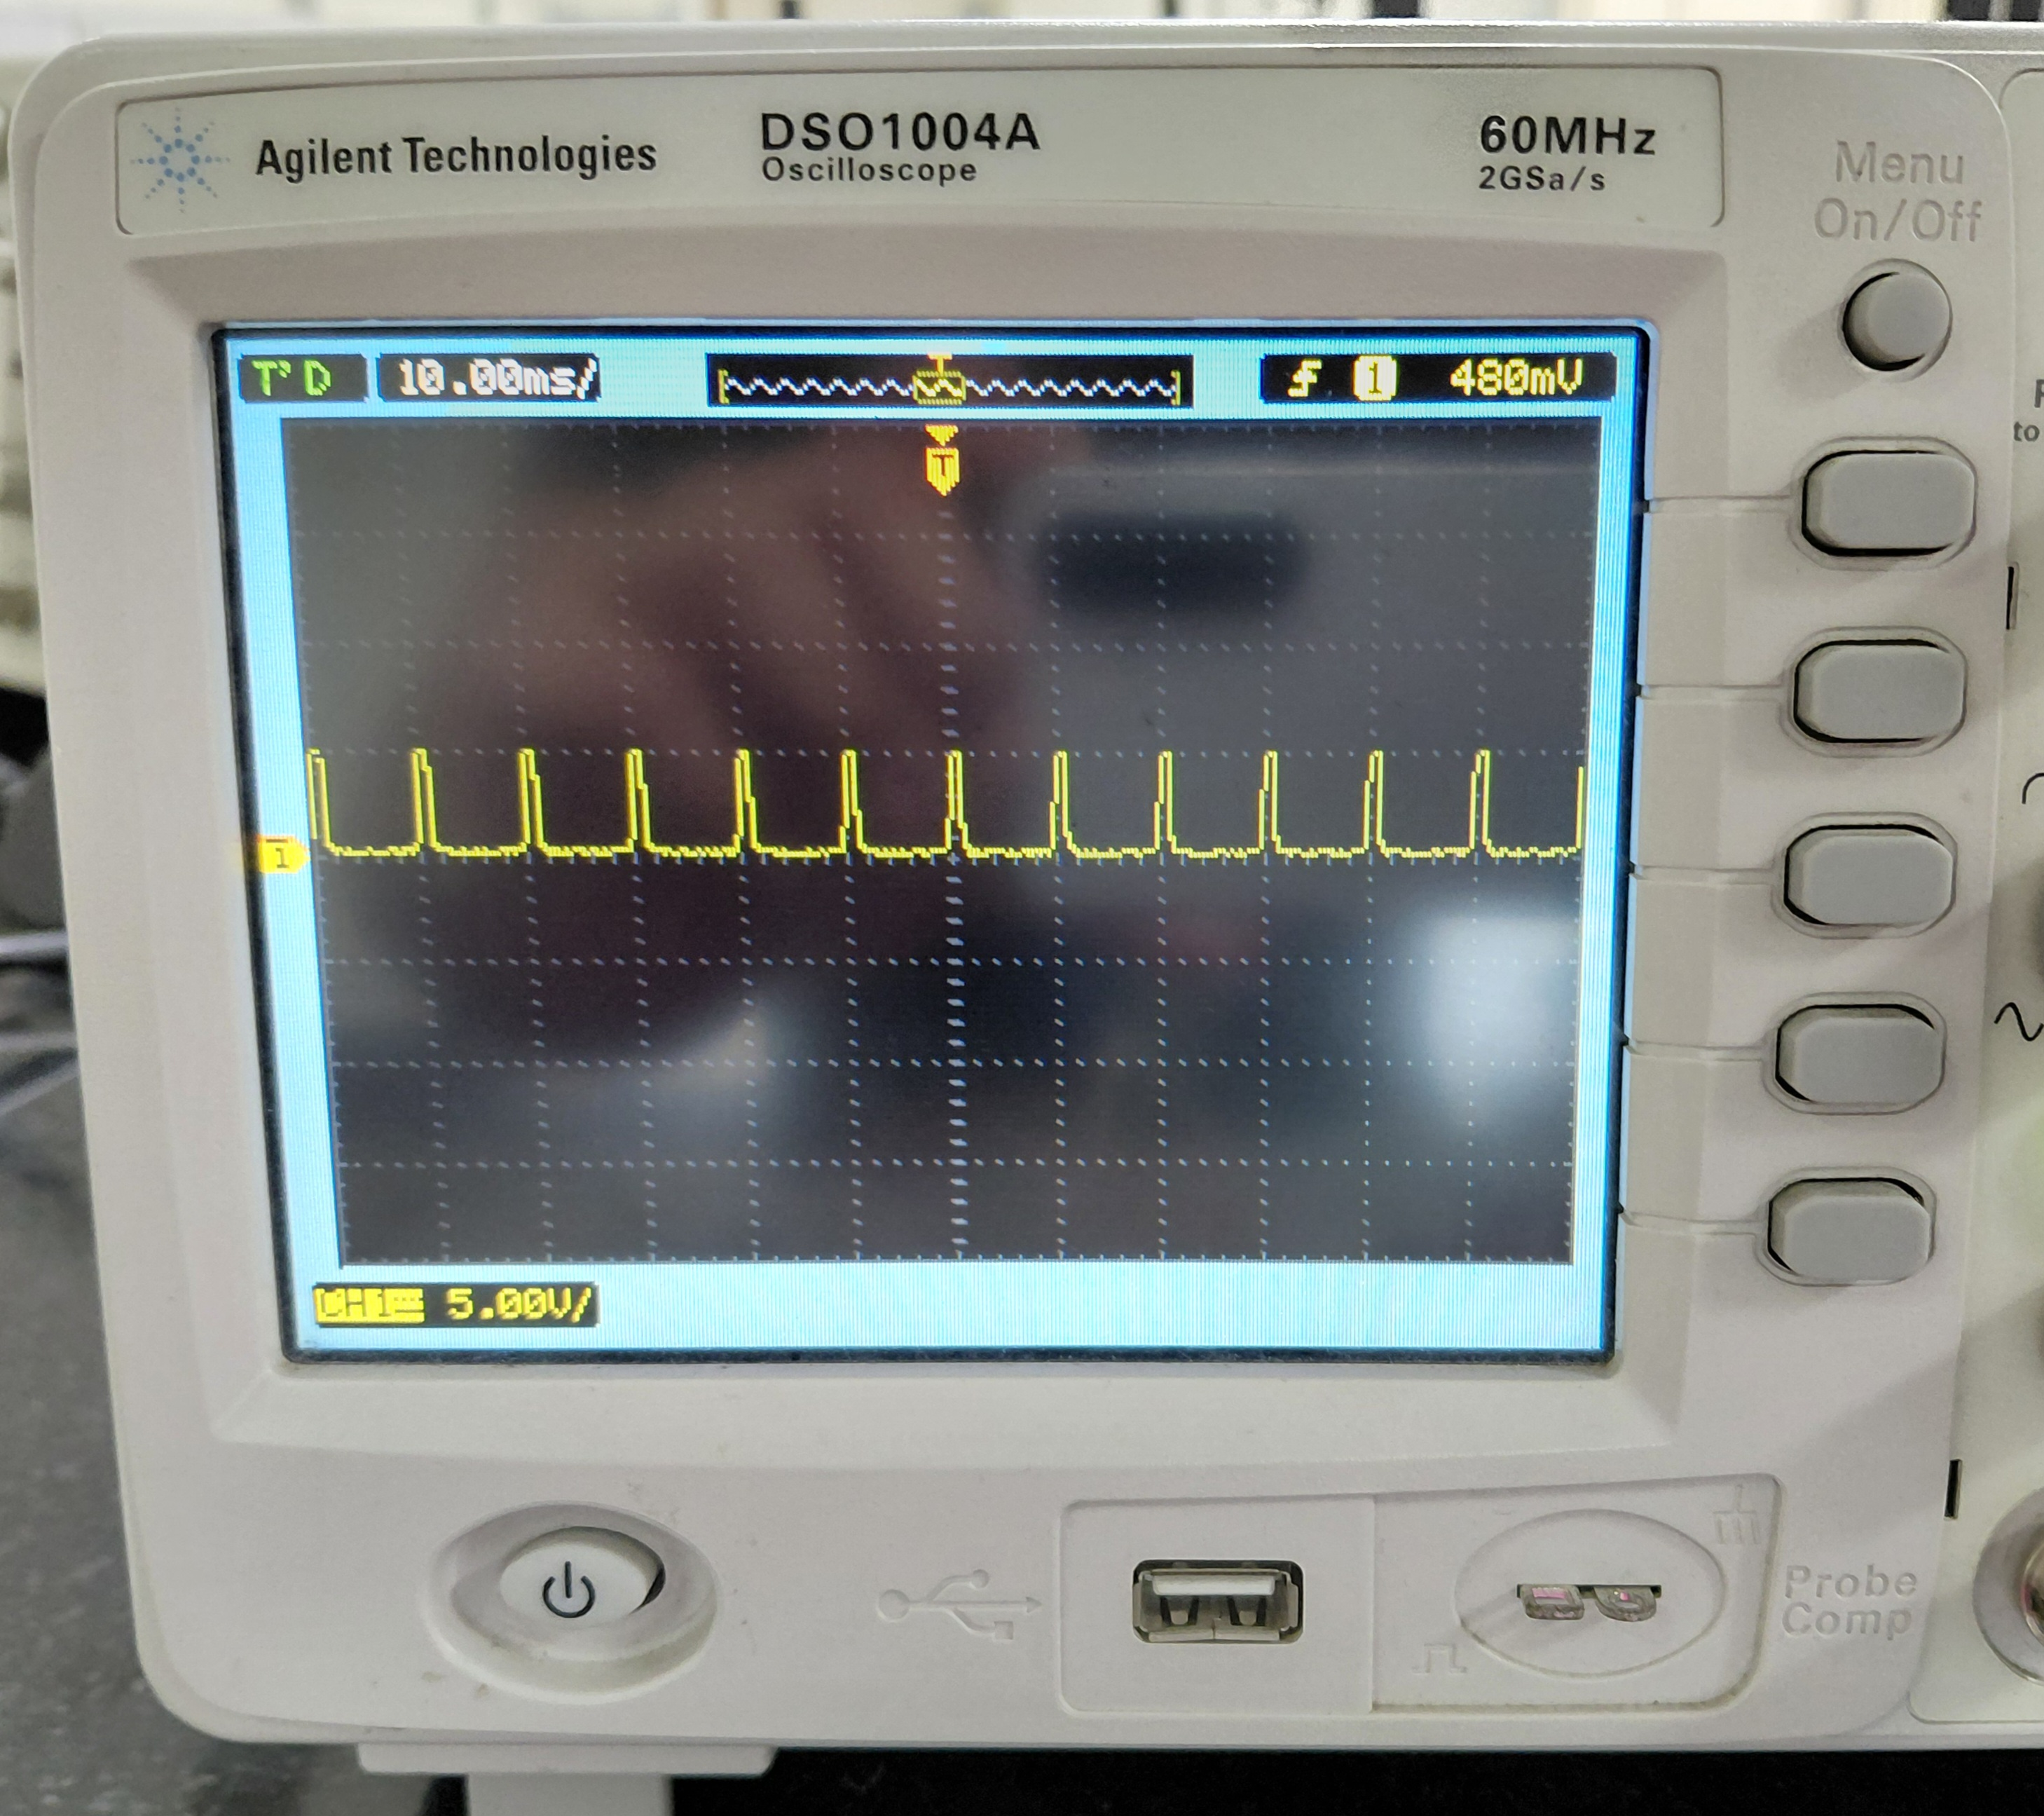
\includegraphics[width=0.5\columnwidth]{20251113_150136 (1).jpg}
	\caption{This is the output for the interrupt signal from the zero-crossing detector being fired. We have a pulse/signal every $\SI{10}{\milli\second}$ as seen on the oscilloscope.}
	\label{fig:interrupt_signal}
\end{figure}

\section{Software}
The code that we've written for the project is in C++, it integrates all hardware components into a single, event-driven closed loop system.

We've have used some libraries for the operation of certain sensors, or simply the PID algorithm.

\begin{enumerate}
	\item \verb|<Wire.h>|: This is for the I2C communication, allowing us to use the \emph{ADS1115} and the LCD Display.

	\item \verb|<Adafruit_ADS1X15.h>|: It's a high level interface, specifically for the \emph{ADS1115} IC. It makes the process of setting a gain, and reading 16-bit analog values easier.

	\item \verb|<PID_v1.h>|: This is our robust, prebuilt PID algorithm, saving us development time.

	\item \verb|<Emonlib.h>|: This is to directly communicate with the \emph{SCT-013-030} current sensor module, when using the Arduino's inbuilt ADC.

	\item \verb|<ZMPT101B.h>|: This is for direct communicationwith the voltage sensing module,when using the Arduino's inbuilt ADC.
\end{enumerate}

We initialized the system with the \verb|setup()| function to configure the components before the main loop. \verb|ads.begin()| and the \verb|ads.setGain(GAIN_ONE)| to start the ADS and configures the full 16-bit resolution over a $\pm \SI{4.096}{\volt}$ range.

\noindent Next thing, we initialize is the PID controller. \verb|myPID.SetSampleTime(100)| tells the PID to run every $\SI{100}{\milli\second}$ and the main PID function is 

\noindent \verb|PID(&measurePower, &pidOutput, &setpointPower, Kp, Ki, Kd, REVERSE)|

A very important part of the code is the interrupt attachment done through: 

\noindent \verb|attachInterrupt(digitalPinToInterrupt(ZCD_PIN), onZeroCross, CHANGE)|. 
It tells the microcontroller to stop whatever it is doing and immediately run the \verb|onZeroCross()|

\noindent The main loop is structured to be non-blocking, ensuring that firing logic is never delayed.
\begin{lstlisting}[language=C++]
if (zcdFlag == true) {
	// Wait for the delay calculated by the PID
	delayMicroseconds(firingDelay);

	// Fire the Triac
	digitalWrite(TRIAC_PIN, HIGH);
	delayMicroseconds(20); // Short pulse
	digitalWrite(TRIAC_PIN, LOW);
	   
	zcdFlag = false; // Reset the flag
}
\end{lstlisting}
\noindent This is the most time-sensitive part of the code. It waits for the \verb|firingDelay| (calculated by the PID controller) and then sends a brief $\SI{20}{\micro\second}$ pulse to the \emph{MOC3023M}, triggering the Triac for that cycle.

Next we calculate the power using \verb|calculatePower()|. We run this function inside a \verb|millis()| timer. We run a \verb|for| loop that takes many sample readings from the ADC. We calculate the RMS value of current and voltage using these readings. And finally, we update the global \verb|measuredPower| variable, which the PID controller use.
\begin{lstlisting}[language=C++]
// --- FUNCTION TO CALCULATE POWER ---
void calculatePower() {
  // Use 64-bit integers to prevent overflow (the 'nan' bug)
  unsigned long long sumVoltageSq = 0;
  unsigned long long sumCurrentSq = 0;
  
  int16_t voltageSample;
  int16_t currentSample;

  for (int i = 0; i < sampleCount; i++) {
    voltageSample = ads.readADC_SingleEnded(VOLT_ADC_S);
    currentSample = ads.readADC_SingleEnded(CURR_ADC_S);

    long filteredVoltage = voltageSample - voltageOffset;
    long filteredCurrent = currentSample - currentOffset;

    sumVoltageSq += (unsigned long long)filteredVoltage*filteredVoltage;
    sumCurrentSq += (unsigned long long)filteredCurrent*filteredCurrent;
  }

  // Calculate RMS Voltage
  double meanVoltageSq = (double)sumVoltageSq / sampleCount;
  double rmsVoltageRaw = sqrt(meanVoltageSq);
  double Vrms = rmsVoltageRaw * ADS_VOLTS_PER_BIT * VOLTAGE_CAL;

  // Calculate RMS Current
  double meanCurrentSq = (double)sumCurrentSq / sampleCount;
  double rmsCurrentRaw = sqrt(meanCurrentSq);
  double Irms = rmsCurrentRaw * ADS_VOLTS_PER_BIT * CURRENT_CAL;

  // Update the global measuredPower variable
  measuredPower = Vrms * Irms;
}
\end{lstlisting}
Inside the same $\SI{100}{\milli\second}$ timer, after the power is calculated, the \verb|myPID.Compute()| function is called. This single command tells the PID library to:
\begin{enumerate}
	\item Read the \verb|measuredPower| (Input).
	\item Compare it to \verb|setpointPower| (Setpoint).
	\item Calculate the error.
	\item Run its internal P, I, and D logic.
	\item Update the \verb|pidOutput| (Output) variable.
\end{enumerate}
Immediately after, the code maps this new output to the \verb|firingDelay|. This mapping is inverted: a low PID output (0, for "min power") results in a long $\SI{9500}{\micro\second}$ delay, and a high PID output (255, for "max power") results in a short $\SI{1000}{\micro\second}$ delay. This is what steers the system toward the setpoint.
\section{Debugging}
\subsection{AC Control Failure}
During initial testing, the load (light bulb) failed to energize, even when the microcontroller sent a trigger signal.
\begin{itemize}
	\item{\textbf{Diagnostics:}} 
		A "Dumb Blinker" test sketch was developed to bypass the zero-crossing detector and trigger the triac blindly at a fixed interval. This isolated the fault to the \emph{MOC3023M}/Triac circuit.
		We verified the load by connecting it directly to mains (Passed). We probed the \emph{MOC3023M} input (Pin 1/2) with a multimeter. The Arduino was correctly delivering 1.2V during the "ON" state (Passed). Finally, we probed the \emph{MOC3023M} output (Pin 4/6). No conduction was detected despite the input signal. (Failed)
	\item{\textbf{Cause:}}
		The \emph{MOC3023M} optocoupler output stage had failed open. Further analysis of the initial soldering revealed that the gate current-limiting resistor ($\SI{470}{\ohm}$) was initially placed incorrectly, likely causing a massive current surge through the phototriac during the first power-up event.
	\item{\textbf{Solution:}}
		The \emph{MOC3023M} was replaced. The wiring was corrected to ensure the $\SI{470}{\ohm}$ resistor was placed strictly in series between the MOC output pin and the triac Gate to limit surge current to safe levels.
\end{itemize}
\subsection{Zero-Crossing Detection Failure}
The synchronization circuit proved to be the most complex subsystem to debug, requiring multiple iterations and component changes. Initially, the ZCD interrupt service routine never triggered, despite correct wiring. A manual examination of the IC revealed that the \emph{H11AA1} IC was dead, and due to unavailibilty of the same chip we obtained a \emph{PC814} IC as replacement. Even with replacement the system failed to achieve phase control. The interrupt service routine was either not firing or firing erratically only during power-on transients.
\begin{itemize}
	\item{\textbf{Diagnostics:}}
		An oscilloscope was used to visualize the analog output of the \emph{ZMPT101B} voltage sensor. We also used a function generator to replicate the signal from the voltage sensor module and then alter it to figure out the point of failure. We needed to overcome the forward voltage ($V_f \approx \SI{1.2}{\volt}$) of the optocoupler's internal LEDs.
	\item{\textbf{Cause:}}
		The signal was found to be biased at $\SI{2.5}{\volt}$ DC. The \emph{PC814} forward voltage was almost always getting exceeded by the signal because the signal oscillated between $\SI{1.5}{\volt}$ and $\SI{4}{\volt}$, it was always higher than $\SI{1.2}{\volt}$. This meant the \emph{PC814} was permanently forward-biased (ON), holding the interrupt pin LOW.
	\item{\textbf{Solution}}
		We replaced the \emph{ZMPT101B} module on the input side and replaced it with a step-down trasnformer of $230\si{\volt}$ to $12\si{\volt}$ kind. We connected the the center tap of the output side to the \emph{PC814} IC and provided a $6\si{\volt}$ peak signal. We also added multiple high wattage resistors before the IC so the signal not exceed the maximum forward current rating.
\end{itemize}
\subsection{Measurement \& ADC Integration}
RMS calculations for voltage and current were inaccurate or returning \verb|nan| (Not a Number) errors.
\begin{itemize}
	\item \textbf{Diagnostics:}
		After running for several seconds, the RMS value would become corrupted.
	\item \textbf{Cause:}
		The \verb|sumVoltageSq| variable, used to accumulate squared ADC samples, was declared as a \verb|long| (32-bit). With 500 samples of 16-bit squared data, the value exceeded the maximum limit ($2.1 \times 10^9$), causing an integer overflow to a negative value. Attempting to calculate the \verb|sqrt()| of this negative number resulted in \verb|nan|.
	\item \textbf{Solution:}
		Accumulator variables were promoted to \verb|unsigned long long| (64-bit) to prevent overflow.
\end{itemize}
\section{Results \& Discussion}
While we aimed to implement a fully integrated, real-time PID control loop, the final execution was constrained by the hardware resources of the microcontroller. However, extensive unit testing successfully validated the electronic design, the measurement accuracy, and the phase-control logic.

Before attempting full integration, individual modules were subjected to rigorous testing to verify their reliability. 
To verify the "Muscle" (\emph{MOC3023M} and \emph{BTA416}) and "Timing" (\emph{PC814} ZCD) circuits, a hard-coded delay test was performed. The system successfully triggered the Triac at precise intervals (e.g., $5000\si{\micro\second}$ after zero-crossing). The load (light bulb) maintained a stable, flicker-free brightness consistent with the firing angle. This confirmed that the ZCD interrupt was firing correctly at $100\si{\hertz}$ and the isolation circuit was functioning safely.
A "Looper" test code was implemented to sweep the firing delay from $1000\si{\micro\second}$ (Max Power) to $9000\si{\micro\second}$ (Min Power) and back. The bulb dimmed and brightened smoothly without stuttering or erratic flashing. This proved that the system could handle dynamic changes in firing angle in real-time, a prerequisite for PID control.
The sensing module was tested using the RMS calculation algorithm. The system successfully calculated \verb|Vrms|, \verb|Irms|, and \verb|Apparent Power|. The readings were compared against standard multimeter values. The 16-bit \emph{ADS1115} provided sufficient resolution to detect small changes in load current, validating the "Feedback" portion of the control loop.

The primary challenge encountered during the final phase was the integration of all software modules onto the Arduino Uno (ATmega328P). The Arduino Uno possesses only 2KB of Dynamic Memory (SRAM). The project required several memory-intensive libraries to run simultaneously. We understand that there might be some clever or more efficient ways to resolve this issue, but due to our groups inexperience in \emph{C++} proved to be a big obstacle in this. We had to chose to restric ourselves to only demonstrate the indivudual components of our project.

The original plan included testing the system with a Variac. By artificially lowering the input voltage (simulating a "brownout"), we intended to prove that the PID loop would automatically decrease the firing delay to maintain constant power at the bulb. Since the full PID loop could not run stably alongside the measurement code, this dynamic compensation could not be empirically verified. This validation test was not conducted at the end due to project timeline and limited resources.

Despite the integration setback, we believe that we have successfully delivered a professional-grade hardware platform. The hardware design, safety isolation features, and sensor calibration methods were proven effective. The electronic hardware is fully capable of supporting closed-loop control; the limitation lies strictly within the computational capacity of the chosen microcontroller.
\end{document}
